% !TeX root = main.tex
\section{数据分析}
\subsection{上海}

本研究搜集了 11681 份上海市住房价格数据, 整理了 35 个区位中心, 如图 \ref{fig:shanghai} 所示.

\begin{figure}[htbp]
  \centering
  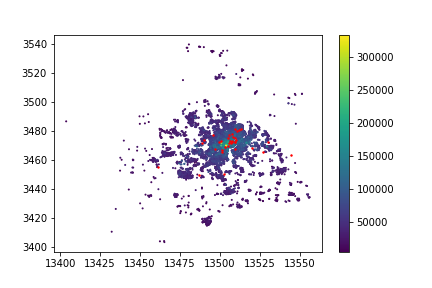
\includegraphics[width=.5\linewidth]{shanghai/shanghai.png}
  \caption{上海市住房价格分布} \label{fig:shanghai}
\end{figure}

其中横纵坐标单位为 \si{\kilo\metre}, 颜色的深浅反映了住房价格的高低, 红色标点表示区块中心所在位置.
使用前文所述的模型进行拟合, 得到结果如表 \ref{tab:shanghai_result} 所示.

使用拟合结果进行预测, 可以得到上海市的住房价格分布预测如图 \ref{fig:shanghai_predict} 所示.

\begin{figure}[htbp]
  \centering
  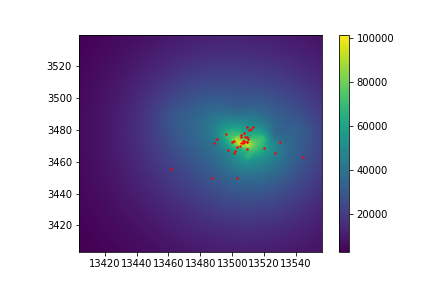
\includegraphics[width=.5\linewidth]{shanghai/shanghai_predict.png}
  \caption{上海市住房价格预测}
  \label{fig:shanghai_predict}
\end{figure}

进一步地, 对区块中心的类型进行统计分析可以得到上海市住房价格受教育, 医疗, 商业等因素的影响, 如图 \ref{fig:shanghai_impact}.
其中影响因子为正表示住房价格随与区位中心距离的缩短而提高.

\begin{figure}[htbp]
  \centering
  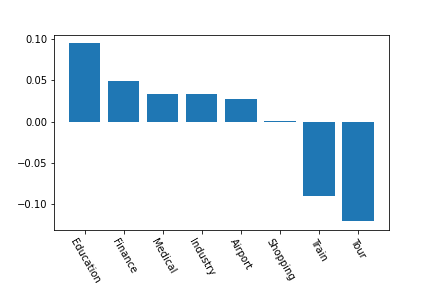
\includegraphics[width=.5\linewidth]{shanghai/shanghai_impact.png}
  \caption{上海市住房价格影响因子}
  \label{fig:shanghai_impact}
\end{figure}
